\fontfamily{\sfdefault}\selectfont
% XCircuit output "aperture_noise.tex" for LaTeX input from aperture_noise.ps
\def\putbox#1#2#3#4{\makebox[0.00000in][l]{\makebox[#1][l]{}\raisebox{\baselineskip}[0.00000in][0.00000in]{\raisebox{#2}[0.00000in][0.00000in]{\scalebox{#3}{#4}}}}}
\def\rightbox#1{\makebox[0.00000in][r]{#1}}
\def\centbox#1{\makebox[0.00000in]{#1}}
\def\topbox#1{\raisebox{-0.60\baselineskip}[0.00000in][0.00000in]{#1}}
\def\midbox#1{\raisebox{-0.20\baselineskip}[0.00000in][0.00000in]{#1}}
   \scalebox{1}{
   \normalsize
   \parbox{2.24062in}{
   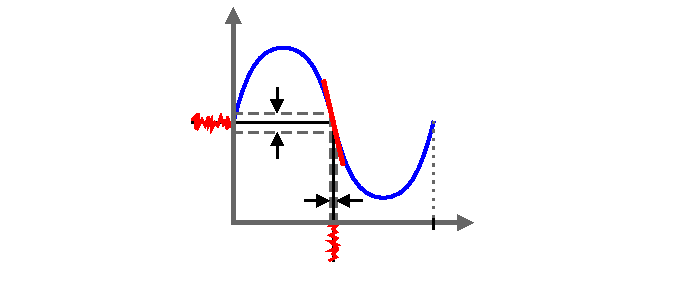
\includegraphics[scale=0.90000]{./figs/aperture_noise.pdf}\\
   % translate x=-108 y=240 scale 0.38
   \putbox{1.87200in}{0.16200in}{0.96}{\rotatebox{-360}{$\Phi$}}%
   \putbox{0.07200in}{1.40400in}{0.96}{V$_{out}$}%
   \putbox{0.63000in}{1.13400in}{0.96}{$\sigma_{v_n}$}%
   \putbox{0.61200in}{0.40500in}{0.96}{$\sigma_{\Phi_n}$}%
   \putbox{0.05400in}{1.06200in}{0.60}{Thermal }%
   \putbox{0.12600in}{0.97200in}{0.60}{noise}%
   \putbox{0.71100in}{0.14400in}{0.60}{Phase }%
   \putbox{0.72900in}{0.05400in}{0.60}{noise}%
   \putbox{1.58400in}{0.14400in}{0.60}{\rotatebox{-360}{$2\pi$}}%
   \putbox{0.40500in}{0.14400in}{0.60}{$0$}%
   } % close 'parbox'
   } % close 'scalebox'
   \vspace{-\baselineskip} % this is not necessary, but looks better
\fontfamily{\rmdefault}\selectfont
